\section{Methods: Omeprazole PBPK model: fit PK}

\subsection{Parameters and data}

15 parameters were optimized: Vmax CYP2C19 S-omeprazole (\texttt{LI\_\_CYP2C19\_Vmax\_some}), Vmax CYP2C19 R-omeprazole (\texttt{LI\_\_CYP2C19\_Vmax\_rome}), Vmax CYP3A4 S-omeprazole (\texttt{LI\_\_CYP3A4\_Vmax\_some}), Vmax CYP3A4 R-omeprazole (\texttt{LI\_\_CYP3A4\_Vmax\_rome}), maximal inactivation rate of CYP2C19 by omeprazole (\texttt{LI\_\_CYP2C19\_kinact}), tissue/plasma partition coefficient omeprazole (\texttt{Kp\_ome}), rate of the gastric emptying and the release of an enteric-coated form (\texttt{GU\_\_Ka\_ec\_ome}), rate of omeprazole absorption (\texttt{GU\_\_OMEABS\_k}), fraction 5-hydroxyomeprazole of the CYP3A4 metabolism of R-omeprazole (\texttt{LI\_\_f\_rome\_cyp3a4\_omeoh}), rate of the 5-hydroxyomeprazole release from the liver (\texttt{LI\_\_OMEOHEX\_k}), renal clearance of 5-hydroxyomeprazole relative to the GFR (\texttt{KI\_\_OMEOHEX\_f}), rate of the CYP2C19 metabolism of omeprazole sulfone (\texttt{LI\_\_OMESUL2C19\_k}), rate of the CYP2C19 independent metabolism of omeprazole sulfone (\texttt{LI\_\_OMESULM\_k}), renal clearance of the other metabolites relative to the GFR (\texttt{KI\_\_OMEOTHEX\_f}) and rate of the biliary excretion of the other metabolites (\texttt{LI\_\_OMEOTHBIL\_k}).

A fit mapping is a curve of a study, the data and the observable of the model it is compared with. The fit has 120 fit mappings of training data with 1285 data points, whose residuals enter the objective; 90 fit mappings of validation data with 845 data points, which were simulated and evaluated with the fitted parameters but not fitted; and 3 fit mappings of outliers with 23 data points, data the fit dropped as not usable, which were evaluated like the validation data so that the decision to drop them can be checked. The fit was set up and run with sbmlsim \cite{Koenig2026_sbmlsim}.

\subsection{Objective function}

The parameters were estimated by minimizing the objective function

\begin{equation}
F(\vec{p}) = \frac{1}{2} \sum_{k} \sum_{i} \rho\left(w_{i,k}\, r_{i,k}(\vec{p})^2\right)
\end{equation}

where $k$ runs over the fit mappings of the training data and $i$ over their data points, $r_{i,k}$ is the residual, $w_{i,k} = w_k\, w^{p}_{i,k}$ the weight of the data point and $\rho$ the loss function, applied to the squared weighted residual $z = w_{i,k}\, r_{i,k}^2$. The loss function is linear, $\rho(z) = z$, i.e. a standard least squares problem.

The residuals are normalized by the mean $\overline{y}_k$ of the data of their curve, which makes curves of different quantities and magnitudes comparable:

\begin{equation}
r_{i,k} = \frac{y_{i,k} - f_k(x_{i,k}, \vec{p})}{\overline{y}_k}
\end{equation}

The weight of curve $k$ is $w_k = n_k / N_k$, the weight $n_k$ of its fit mapping (the weight its fit mapping collection assigns, 1 by default, or, for a collection which uses the weights of its mappings, the weight of the mapping, by default the number of subjects of its data) divided by the number $N_k$ of its data points.

A data point is weighted with the inverse of its coefficient of variation, $w^{p}_{i,k} = |y_{i,k}| / \sigma_{i,k}$, with $\sigma_{i,k}$ the standard deviation of the data point, or its standard error for data without a standard deviation. An error of zero is missing, a missing error of a curve with errors is replaced by the largest error of the curve, and the data points of a curve without errors have the weight $w^{p}_{i,k} = 2$, the weight of a coefficient of variation of 0.5.

\subsection{Optimization}

The optimizer searched the parameters in log10 space within their bounds; bounds, values and intervals are given in the units of the fit parameters, the units of the table of the parameters.

The objective was minimized in 5 runs with the trust region reflective method \cite{Branch1999} of the least squares optimizer of SciPy \cite{Virtanen2020}, with a Jacobian of finite forward differences with the relative step 0.05. A run stopped at the tolerances of the change of the cost, of the parameters and of the gradient, ftol = $10^{-8}$, xtol = $10^{-8}$ and gtol = $10^{-8}$.

The start values of the runs were drawn by latin hypercube sampling \cite{McKay1979} log-uniformly, i.e. uniformly in the logarithm of the parameters, within their bounds, with the seed 1234.

The convergence of the runs was assessed from the traces of their cost and the waterfall plot of their final costs, and the parameter set with the lowest cost was used.

The models were simulated with libRoadRunner \cite{Welsh2023} and its integrator CVODE \cite{Hindmarsh2005} with the relative tolerance $10^{-6}$ and the absolute tolerances $10^{-11}$ of an amount, $10^{-11}$ of a concentration and $10^{-7}$ of the other states, which for a species in a concentration is multiplied by the initial volume of its compartment. It ran with the variable step size of libRoadRunner, i.e. with an output at every step of the integrator. A data point at the time of a change after the start of a simulation, e.g. a dose or the reset of a collection, was compared with the state before the change, except the first data point of a curve with data at later times, which starts a collection and was compared with the state after the change.

\subsection{Goodness of fit}

The goodness of fit is given per kind of data (training data, validation data and outliers) by metrics over its $n$ data points with the residuals $e_i = y_i - f(x_i, \hat{\vec{p}})$ at the fitted parameters $\hat{\vec{p}}$, the mean squared error, its root and the root mean squared error normalized by the mean $\overline{y}_{k(i)}$ of the data of the curve of a point:

\begin{equation}
\mathrm{MSE} = \frac{1}{n} \sum_{i=1}^{n} e_i^2, \quad \mathrm{RMSE} = \sqrt{\mathrm{MSE}}, \quad \mathrm{NRMSE} = \sqrt{\frac{1}{n} \sum_{i=1}^{n} \left(\frac{e_i}{\overline{y}_{k(i)}}\right)^2}
\end{equation}

The root mean square of the residuals of the objective, i.e. what the fit minimizes, and the coefficient of determination:

\begin{equation}
\mathrm{RMSE}_w = \sqrt{\frac{1}{n} \sum_{i=1}^{n} \rho\left(w_i\, r_i^2\right)}, \quad R^2 = 1 - \frac{\sum_{i} e_i^2}{\sum_{i} \left(y_i - \overline{y}\right)^2}
\end{equation}

The predictions of a non-linear model are no linear regression of the data, so $R^2$ can be negative: the prediction is worse than the mean of the data. The information criteria of Akaike \cite{Akaike1974} and Schwarz \cite{Schwarz1978} with the number $n_p$ of fitted parameters are those of a least squares fit with normally distributed residuals, up to an additive constant, so only differences between models fitted to the same data are meaningful:

\begin{equation}
\mathrm{AIC} = n \ln(\mathrm{MSE}) + 2 n_p, \quad \mathrm{BIC} = n \ln(\mathrm{MSE}) + n_p \ln(n)
\end{equation}

The percentage of the data points whose prediction $f_i = f(x_i, \hat{\vec{p}})$ lies within twofold of the data is taken over the $n_+$ data points with positive data $y_i > 0$ and a positive prediction $f_i > 0$; the others have no ratio and are not counted, and a kind of data without such a point has no percentage:

\begin{equation}
P_2 = \frac{100}{n_+} \left|\left\{ i : \frac{1}{2} \le \frac{f_i}{y_i} \le 2 \right\}\right|
\end{equation}

The goodness of fit plot shows the predictions against the data on logarithmic axes, with the lines of twofold $f = 2y$ and $f = y/2$. The Bland-Altman plot \cite{Bland1986} shows the ratio of prediction and data as $d_i = \log_{10}(f_i / y_i)$ against the geometric mean $\sqrt{f_i\, y_i}$ for the data points with positive values, with the bias $\overline{d}$ and the limits of agreement $\overline{d} \pm 1.96\, s_d$, with the sample standard deviation $s_d$ of $d_i$, of the training data; they are read as the fold factors $10^{\overline{d}}$ and $10^{\overline{d} \pm 1.96\, s_d}$.

\subsection{Identifiability}

The identifiability of the parameters was analysed with the profile likelihood \cite{Raue2009,Kreutz2013}. The profile of a parameter is the lowest objective with the parameter fixed:

\begin{equation}
\mathrm{PL}(p_j) = \min_{p_{l \neq j}} F(\vec{p})
\end{equation}

At every point of a scan the other parameters were re-optimized from the previous point with the least squares optimizer of SciPy with the relative step 0.05. A scan ran from the optimum in both directions in the space of the optimizer, with steps in decades of the parameter, starting at 0.1. A step which raised the objective by more than 0.2 of the distance between the objective at the optimum and the threshold was reduced by the factor 2 and repeated, down to 0.01, and the step after one which raised it by less than that divided by the factor was enlarged by the factor, up to 1. A scan stopped at the threshold, at the bound of the parameter, at a point which failed or after 50 points.

The confidence intervals are the values at which the profile crosses the threshold of the likelihood ratio test

\begin{equation}
F_{\mathrm{thr}} = F_{\min} + \frac{\chi^2_{\alpha}(\mathrm{df})}{2}
\end{equation}

with $F_{\min}$ the lowest objective of the fit and of all profiles and $\chi^2_{\alpha}(\mathrm{df})$ the quantile of the $\chi^2$ distribution at the confidence level $\alpha = 0.95$ with df = 1 degrees of freedom, i.e. 1.92 above the lowest objective. The threshold has this confidence level if $F$ is the negative log-likelihood of the data up to a constant, i.e. if the weighted residuals are independent and normally distributed with unit variance; otherwise the level is approximate. A crossing is interpolated between two points of the profile, on the logarithm of a parameter on a logarithmic scale. A parameter is identifiable if its profile reaches the threshold within the scan on both sides of the optimum, i.e. its confidence interval is finite; practically non-identifiable towards the lower bound if its profile reaches the threshold above the optimum but not below it within the scan, which ends at the lower bound or after 50 points; practically non-identifiable towards the upper bound if its profile reaches the threshold below the optimum but not above it within the scan, which ends at the upper bound or after 50 points; practically non-identifiable if its profile reaches the threshold on neither side within the scans, which end at the bounds or after 50 points, and is not flat; and structurally non-identifiable if its profile is flat on both sides. A side of a profile is flat if it rises by less than 0.05 of the distance between the lowest objective and the threshold, and a profile with a point which failed or did not converge is not classified. The profile likelihood is preferred over the intervals of the Fisher information, its intervals are invariant under a transformation of the parameters and can be asymmetric \cite{Wieland2021}.

The Fisher information is the local alternative to the profiles: it is the Gauss-Newton approximation of the curvature of the objective at the optimum, from the Jacobian $J$ of the weighted residuals of the training data with respect to the parameters $\vec{p}$ in the space of the optimizer, computed by central finite differences with the step $h_j = \epsilon \max(|p_j|, 1),\ \epsilon = 10^{-6}$ of the parameter $p_j$:

\begin{equation}
I = J^\top J, \quad \mathrm{cov} = \sigma^2 I^{-1}, \quad \sigma^2 = \frac{2 F}{n - n_p}
\end{equation}

with the number $n$ of data points of the training data and the number $n_p$ of parameters. The information has rank 15 of 15, the number of its eigenvalues above $10^{-8}$ of the largest one, and the condition number 551; the covariance of an information of a lower rank is computed with the pseudo-inverse. The Wald intervals are $\hat{p}_j \pm t_{(1+\alpha)/2,\, n-n_p}\, \mathrm{SE}_j$ with the standard errors $\mathrm{SE}_j = \sqrt{\mathrm{cov}_{jj}}$ at the confidence level $\alpha = 0.95$, transformed back into the units of the fit parameters.

\subsection{Provenance}

The fit PK\_20261020\_090631\_\_aa2cf was run on 2026-10-20 07:06:37 UTC with sbmlsim 0.10.0 \cite{Koenig2026_sbmlsim}, libRoadRunner 2.10.0 \cite{Welsh2023}, SciPy 1.18.1 \cite{Virtanen2020}, NumPy 2.5.3 \cite{Harris2020} and Python 3.14.4 (seed 1234). The models and data were those of commit \texttt{12acae3ea6826f839295cf826fbb82a2f81d24bd} of \texttt{/home/mkoenig/git/pkdb\_models-omeprazole}; their SHA-256 checksums are listed in Table~\ref{tab:checksums:PK_20261020_090631__aa2cf}.

\begin{longtable}{ll}
\caption{SHA-256 checksums of the models and data of the fit PK\_20261020\_090631\_\_aa2cf, their first 12 characters; the full checksums are in the provenance of the result (optimization\_result.json).}\label{tab:checksums:PK_20261020_090631__aa2cf} \\
\toprule
File & SHA-256 \\
\midrule
\endfirsthead
\multicolumn{2}{l}{\small\tablename~\thetable{} (continued)} \\
\toprule
File & SHA-256 \\
\midrule
\endhead
\bottomrule
\endlastfoot
\texttt{pkdb\_models/models/omeprazole/data/caffeine/Oh2012/.Oh2012\_Fig3.tsv} & \texttt{e7458fb27a6d...} \\
\texttt{pkdb\_models/models/omeprazole/data/caffeine/Oh2012/.Oh2012\_TabGroups.tsv} & \texttt{021f55009aad...} \\
\texttt{pkdb\_models/models/omeprazole/data/caffeine/Oh2012/.Oh2012\_TabInterventions.tsv} & \texttt{2ccc461e26f0...} \\
\texttt{pkdb\_models/models/omeprazole/data/omeprazole/Andersson1990/.Andersson1990\_Fig1.tsv} & \texttt{733dc8a41711...} \\
\texttt{pkdb\_models/models/omeprazole/data/omeprazole/Andersson1990/.Andersson1990\_Fig1\_mean.tsv} & \texttt{ea59f930d42e...} \\
\texttt{pkdb\_models/models/omeprazole/data/omeprazole/Andersson1990/.Andersson1990\_Fig1\_median.tsv} & \texttt{687ea78cf6a8...} \\
\texttt{pkdb\_models/models/omeprazole/data/omeprazole/Andersson1990/.Andersson1990\_Fig2.tsv} & \texttt{4cac47c8174d...} \\
\texttt{pkdb\_models/models/omeprazole/data/omeprazole/Andersson1990/.Andersson1990\_Fig2\_mean.tsv} & \texttt{77b4f8b6da2b...} \\
\texttt{pkdb\_models/models/omeprazole/data/omeprazole/Andersson1990/.Andersson1990\_Fig2\_median.tsv} & \texttt{4c5f0431c4f1...} \\
\texttt{pkdb\_models/models/omeprazole/data/omeprazole/Andersson1990/.Andersson1990\_Fig3.tsv} & \texttt{e3d522280e61...} \\
\texttt{pkdb\_models/models/omeprazole/data/omeprazole/Andersson1990/.Andersson1990\_Fig3\_mean.tsv} & \texttt{65df4647ec2f...} \\
\texttt{pkdb\_models/models/omeprazole/data/omeprazole/Andersson1990/.Andersson1990\_Fig3\_median.tsv} & \texttt{b27a2249ffd0...} \\
\texttt{pkdb\_models/models/omeprazole/data/omeprazole/Andersson1990/.Andersson1990\_Tab1.tsv} & \texttt{1342c2076d29...} \\
\texttt{pkdb\_models/models/omeprazole/data/omeprazole/Andersson1990/.Andersson1990\_Tab1\_mean.tsv} & \texttt{a1f415bf2505...} \\
\texttt{pkdb\_models/models/omeprazole/data/omeprazole/Andersson1990/.Andersson1990\_Tab2.tsv} & \texttt{edbd312ef2e8...} \\
\texttt{pkdb\_models/models/omeprazole/data/omeprazole/Andersson1990/.Andersson1990\_Tab2\_mean.tsv} & \texttt{f87433b30782...} \\
\texttt{pkdb\_models/models/omeprazole/data/omeprazole/Andersson1990/.Andersson1990\_Tab3.tsv} & \texttt{c3c523840b95...} \\
\texttt{pkdb\_models/models/omeprazole/data/omeprazole/Andersson1990/.Andersson1990\_Tab3\_mean.tsv} & \texttt{cca03a0ed8f7...} \\
\texttt{pkdb\_models/models/omeprazole/data/omeprazole/Andersson1990/.Andersson1990\_TabGroups.tsv} & \texttt{bffec9ca92e5...} \\
\texttt{pkdb\_models/models/omeprazole/data/omeprazole/Andersson1990/.Andersson1990\_TabIndividuals.tsv} & \texttt{308e3dc84b99...} \\
\texttt{pkdb\_models/models/omeprazole/data/omeprazole/Andersson1990/.Andersson1990\_TabInterventions.tsv} & \texttt{93ec1239c8a1...} \\
\texttt{pkdb\_models/models/omeprazole/data/omeprazole/Andersson1990a/.Andersson1990a\_Fig1.tsv} & \texttt{d86c145aa9a7...} \\
\texttt{pkdb\_models/models/omeprazole/data/omeprazole/Andersson1990a/.Andersson1990a\_Tab1.tsv} & \texttt{5045cbd2099b...} \\
\texttt{pkdb\_models/models/omeprazole/data/omeprazole/Andersson1990a/.Andersson1990a\_Tab2.tsv} & \texttt{44cc61e8f14b...} \\
\texttt{pkdb\_models/models/omeprazole/data/omeprazole/Andersson1990a/.Andersson1990a\_TabGroups.tsv} & \texttt{cdfa0f5b7c94...} \\
\texttt{pkdb\_models/models/omeprazole/data/omeprazole/Andersson1990a/.Andersson1990a\_TabInterventions.tsv} & \texttt{a18c062064f3...} \\
\texttt{pkdb\_models/models/omeprazole/data/omeprazole/Andersson1993/.Andersson1993\_Fig1.tsv} & \texttt{1bf73adde56b...} \\
\texttt{pkdb\_models/models/omeprazole/data/omeprazole/Andersson1993/.Andersson1993\_Fig2.tsv} & \texttt{e57d3aa3a541...} \\
\texttt{pkdb\_models/models/omeprazole/data/omeprazole/Andersson1993/.Andersson1993\_Fig3.tsv} & \texttt{e2228662edbb...} \\
\texttt{pkdb\_models/models/omeprazole/data/omeprazole/Andersson1993/.Andersson1993\_Tab2.tsv} & \texttt{a3af1cf1d0c0...} \\
\texttt{pkdb\_models/models/omeprazole/data/omeprazole/Andersson1993/.Andersson1993\_Tab2\_mean.tsv} & \texttt{a291f032fa5a...} \\
\texttt{pkdb\_models/models/omeprazole/data/omeprazole/Andersson1993/.Andersson1993\_Tab3.tsv} & \texttt{e092565a8b64...} \\
\texttt{pkdb\_models/models/omeprazole/data/omeprazole/Andersson1993/.Andersson1993\_Tab3\_mean.tsv} & \texttt{bc4878374204...} \\
\texttt{pkdb\_models/models/omeprazole/data/omeprazole/Andersson1993/.Andersson1993\_TabGroups.tsv} & \texttt{0bdd6bda88de...} \\
\texttt{pkdb\_models/models/omeprazole/data/omeprazole/Andersson1993/.Andersson1993\_TabIndividuals.tsv} & \texttt{a3287bc78589...} \\
\texttt{pkdb\_models/models/omeprazole/data/omeprazole/Andersson1993/.Andersson1993\_TabInterventions.tsv} & \texttt{bc562a03a322...} \\
\texttt{pkdb\_models/models/omeprazole/data/omeprazole/Andersson2001/.Andersson2001\_Fig2.tsv} & \texttt{0de2b5bae4e7...} \\
\texttt{pkdb\_models/models/omeprazole/data/omeprazole/Andersson2001/.Andersson2001\_Fig9.tsv} & \texttt{dfc99cbbaca3...} \\
\texttt{pkdb\_models/models/omeprazole/data/omeprazole/Andersson2001/.Andersson2001\_TabGroups.tsv} & \texttt{c852015ec95b...} \\
\texttt{pkdb\_models/models/omeprazole/data/omeprazole/Andersson2001/.Andersson2001\_TabInterventions.tsv} & \texttt{63b3e40b01e7...} \\
\texttt{pkdb\_models/models/omeprazole/data/omeprazole/Cederberg1992/.Cederberg1992\_Fig2.tsv} & \texttt{5b8f1d8b6e05...} \\
\texttt{pkdb\_models/models/omeprazole/data/omeprazole/Cederberg1992/.Cederberg1992\_Fig4.tsv} & \texttt{c24afaad3f22...} \\
\texttt{pkdb\_models/models/omeprazole/data/omeprazole/Cederberg1992/.Cederberg1992\_Tab2.tsv} & \texttt{dfc3d87120a1...} \\
\texttt{pkdb\_models/models/omeprazole/data/omeprazole/Cederberg1992/.Cederberg1992\_TabGroups.tsv} & \texttt{e68a11e3be26...} \\
\texttt{pkdb\_models/models/omeprazole/data/omeprazole/Cederberg1992/.Cederberg1992\_TabInterventions.tsv} & \texttt{cf422d7ebeb6...} \\
\texttt{pkdb\_models/models/omeprazole/data/omeprazole/Elkoshi2002/.Elkoshi2002\_Fig1.tsv} & \texttt{36c47e8d0249...} \\
\texttt{pkdb\_models/models/omeprazole/data/omeprazole/Elkoshi2002/.Elkoshi2002\_Fig2.tsv} & \texttt{dbc6f87ef3b9...} \\
\texttt{pkdb\_models/models/omeprazole/data/omeprazole/Elkoshi2002/.Elkoshi2002\_Tab2.tsv} & \texttt{571cffa03282...} \\
\texttt{pkdb\_models/models/omeprazole/data/omeprazole/Elkoshi2002/.Elkoshi2002\_Tab3.tsv} & \texttt{0ad028a91282...} \\
\texttt{pkdb\_models/models/omeprazole/data/omeprazole/Elkoshi2002/.Elkoshi2002\_Tab4.tsv} & \texttt{57ce0419b165...} \\
\texttt{pkdb\_models/models/omeprazole/data/omeprazole/Elkoshi2002/.Elkoshi2002\_TabGroups.tsv} & \texttt{779470e0b21d...} \\
\texttt{pkdb\_models/models/omeprazole/data/omeprazole/Elkoshi2002/.Elkoshi2002\_TabInterventions.tsv} & \texttt{f5c953607d01...} \\
\texttt{pkdb\_models/models/omeprazole/data/omeprazole/Faruquee2010/.Faruquee2010\_Fig1.tsv} & \texttt{e4a7944ad03f...} \\
\texttt{pkdb\_models/models/omeprazole/data/omeprazole/Faruquee2010/.Faruquee2010\_Fig2.tsv} & \texttt{f1f441f18ece...} \\
\texttt{pkdb\_models/models/omeprazole/data/omeprazole/Faruquee2010/.Faruquee2010\_Fig3.tsv} & \texttt{06ec6b48cd90...} \\
\texttt{pkdb\_models/models/omeprazole/data/omeprazole/Faruquee2010/.Faruquee2010\_Fig4.tsv} & \texttt{792ebba18675...} \\
\texttt{pkdb\_models/models/omeprazole/data/omeprazole/Faruquee2010/.Faruquee2010\_Tab1.tsv} & \texttt{aae1a98395a5...} \\
\texttt{pkdb\_models/models/omeprazole/data/omeprazole/Faruquee2010/.Faruquee2010\_Tab2.tsv} & \texttt{7ba9ab397ecc...} \\
\texttt{pkdb\_models/models/omeprazole/data/omeprazole/Faruquee2010/.Faruquee2010\_TabGroups.tsv} & \texttt{07f012ec2d7d...} \\
\texttt{pkdb\_models/models/omeprazole/data/omeprazole/Faruquee2010/.Faruquee2010\_TabInterventions.tsv} & \texttt{7e686fb89ba9...} \\
\texttt{pkdb\_models/models/omeprazole/data/omeprazole/Geus2000/.Geus2000\_Fig2.tsv} & \texttt{711fd442c808...} \\
\texttt{pkdb\_models/models/omeprazole/data/omeprazole/Geus2000/.Geus2000\_Fig3.tsv} & \texttt{89615a25817c...} \\
\texttt{pkdb\_models/models/omeprazole/data/omeprazole/Geus2000/.Geus2000\_Fig4.tsv} & \texttt{9809665d1841...} \\
\texttt{pkdb\_models/models/omeprazole/data/omeprazole/Geus2000/.Geus2000\_Tab1.tsv} & \texttt{578ea8607562...} \\
\texttt{pkdb\_models/models/omeprazole/data/omeprazole/Geus2000/.Geus2000\_Tab2.tsv} & \texttt{77451bd8395d...} \\
\texttt{pkdb\_models/models/omeprazole/data/omeprazole/Geus2000/.Geus2000\_TabGroups.tsv} & \texttt{9bb3fd29c4e5...} \\
\texttt{pkdb\_models/models/omeprazole/data/omeprazole/Geus2000/.Geus2000\_TabIndividuals.tsv} & \texttt{262bc100a4c7...} \\
\texttt{pkdb\_models/models/omeprazole/data/omeprazole/Geus2000/.Geus2000\_TabInterventions.tsv} & \texttt{42ebbb5f5741...} \\
\texttt{pkdb\_models/models/omeprazole/data/omeprazole/HassanAlin2000/.HassanAlin2000\_Fig1.tsv} & \texttt{0cc29edf35fb...} \\
\texttt{pkdb\_models/models/omeprazole/data/omeprazole/HassanAlin2000/.HassanAlin2000\_Fig2.tsv} & \texttt{822169f74716...} \\
\texttt{pkdb\_models/models/omeprazole/data/omeprazole/HassanAlin2000/.HassanAlin2000\_Tab1.tsv} & \texttt{da6decc19286...} \\
\texttt{pkdb\_models/models/omeprazole/data/omeprazole/HassanAlin2000/.HassanAlin2000\_Tab2.tsv} & \texttt{c00b8ee74fe7...} \\
\texttt{pkdb\_models/models/omeprazole/data/omeprazole/HassanAlin2000/.HassanAlin2000\_Tab3.tsv} & \texttt{2d14c7e90dfe...} \\
\texttt{pkdb\_models/models/omeprazole/data/omeprazole/HassanAlin2000/.HassanAlin2000\_TabGroups.tsv} & \texttt{04c61223eb11...} \\
\texttt{pkdb\_models/models/omeprazole/data/omeprazole/HassanAlin2000/.HassanAlin2000\_TabInterventions.tsv} & \texttt{3e87950c58e6...} \\
\texttt{pkdb\_models/models/omeprazole/data/omeprazole/HassanAlin2005/.HassanAlin2005\_Fig1.tsv} & \texttt{d02f2613b009...} \\
\texttt{pkdb\_models/models/omeprazole/data/omeprazole/HassanAlin2005/.HassanAlin2005\_Fig2.tsv} & \texttt{f8c8ed6b4535...} \\
\texttt{pkdb\_models/models/omeprazole/data/omeprazole/HassanAlin2005/.HassanAlin2005\_Tab1.tsv} & \texttt{7e3494e8cdbe...} \\
\texttt{pkdb\_models/models/omeprazole/data/omeprazole/HassanAlin2005/.HassanAlin2005\_Tab2.tsv} & \texttt{7031b3f194db...} \\
\texttt{pkdb\_models/models/omeprazole/data/omeprazole/HassanAlin2005/.HassanAlin2005\_Tab3.tsv} & \texttt{ff12f22559cf...} \\
\texttt{pkdb\_models/models/omeprazole/data/omeprazole/HassanAlin2005/.HassanAlin2005\_Tab4.tsv} & \texttt{1174f953b86a...} \\
\texttt{pkdb\_models/models/omeprazole/data/omeprazole/HassanAlin2005/.HassanAlin2005\_TabGroups.tsv} & \texttt{c7934b41c825...} \\
\texttt{pkdb\_models/models/omeprazole/data/omeprazole/HassanAlin2005/.HassanAlin2005\_TabInterventions.tsv} & \texttt{81e0d00c8d4b...} \\
\texttt{pkdb\_models/models/omeprazole/data/omeprazole/Howden1984/.Howden1984\_Tab1.tsv} & \texttt{95fb9ab26205...} \\
\texttt{pkdb\_models/models/omeprazole/data/omeprazole/Howden1984/.Howden1984\_TabGroup.tsv} & \texttt{c27087bfbc94...} \\
\texttt{pkdb\_models/models/omeprazole/data/omeprazole/Howden1984/.Howden1984\_TabGroups.tsv} & \texttt{08c85511e3cf...} \\
\texttt{pkdb\_models/models/omeprazole/data/omeprazole/Howden1984/.Howden1984\_TabIndividuals.tsv} & \texttt{59642167921d...} \\
\texttt{pkdb\_models/models/omeprazole/data/omeprazole/Howden1984/.Howden1984\_TabIntervention.tsv} & \texttt{2a43ba037cee...} \\
\texttt{pkdb\_models/models/omeprazole/data/omeprazole/Howden1984/.Howden1984\_TabInterventions.tsv} & \texttt{92f052eae202...} \\
\texttt{pkdb\_models/models/omeprazole/data/omeprazole/Howden1984a/.Howden1984a\_Tab1.tsv} & \texttt{680730073e41...} \\
\texttt{pkdb\_models/models/omeprazole/data/omeprazole/Howden1984a/.Howden1984a\_Tab2.tsv} & \texttt{f709074928af...} \\
\texttt{pkdb\_models/models/omeprazole/data/omeprazole/Howden1984a/.Howden1984a\_TabGroups.tsv} & \texttt{4cef141f8db3...} \\
\texttt{pkdb\_models/models/omeprazole/data/omeprazole/Howden1984a/.Howden1984a\_TabIndividuals.tsv} & \texttt{e317b7a1f23e...} \\
\texttt{pkdb\_models/models/omeprazole/data/omeprazole/Howden1984a/.Howden1984a\_TabInterventions.tsv} & \texttt{4d5acf46c687...} \\
\texttt{pkdb\_models/models/omeprazole/data/omeprazole/Iftikhar2024/.Iftikhar2024\_Fig1.tsv} & \texttt{2a1878c44a77...} \\
\texttt{pkdb\_models/models/omeprazole/data/omeprazole/Iftikhar2024/.Iftikhar2024\_Fig2.tsv} & \texttt{c334acb78f84...} \\
\texttt{pkdb\_models/models/omeprazole/data/omeprazole/Iftikhar2024/.Iftikhar2024\_Fig3.tsv} & \texttt{43916f1b89d5...} \\
\texttt{pkdb\_models/models/omeprazole/data/omeprazole/Iftikhar2024/.Iftikhar2024\_Fig4.tsv} & \texttt{a44c2d98397b...} \\
\texttt{pkdb\_models/models/omeprazole/data/omeprazole/Iftikhar2024/.Iftikhar2024\_Tab1.tsv} & \texttt{e1997523387b...} \\
\texttt{pkdb\_models/models/omeprazole/data/omeprazole/Iftikhar2024/.Iftikhar2024\_Tab2.tsv} & \texttt{ed878d60606a...} \\
\texttt{pkdb\_models/models/omeprazole/data/omeprazole/Iftikhar2024/.Iftikhar2024\_Tab3.tsv} & \texttt{215cc856a62c...} \\
\texttt{pkdb\_models/models/omeprazole/data/omeprazole/Iftikhar2024/.Iftikhar2024\_Tab4.tsv} & \texttt{36e0c8c84270...} \\
\texttt{pkdb\_models/models/omeprazole/data/omeprazole/Iftikhar2024/.Iftikhar2024\_TabGroups.tsv} & \texttt{0a60471e0f62...} \\
\texttt{pkdb\_models/models/omeprazole/data/omeprazole/Iftikhar2024/.Iftikhar2024\_TabIndividuals.tsv} & \texttt{e27ea3a19b62...} \\
\texttt{pkdb\_models/models/omeprazole/data/omeprazole/Iftikhar2024/.Iftikhar2024\_TabInterventions.tsv} & \texttt{6d5e6caa25b5...} \\
\texttt{pkdb\_models/models/omeprazole/data/omeprazole/Kita2001/.Kita2001\_Fig1.tsv} & \texttt{9c9a03a32c63...} \\
\texttt{pkdb\_models/models/omeprazole/data/omeprazole/Kita2001/.Kita2001\_Tab1.tsv} & \texttt{6299f21d961c...} \\
\texttt{pkdb\_models/models/omeprazole/data/omeprazole/Kita2001/.Kita2001\_Tab2.tsv} & \texttt{10ab0b403690...} \\
\texttt{pkdb\_models/models/omeprazole/data/omeprazole/Kita2001/.Kita2001\_TabGroups.tsv} & \texttt{55086cbe890f...} \\
\texttt{pkdb\_models/models/omeprazole/data/omeprazole/Kita2001/.Kita2001\_TabIndividuals.tsv} & \texttt{96bd7935f55b...} \\
\texttt{pkdb\_models/models/omeprazole/data/omeprazole/Kita2001/.Kita2001\_TabInterventions.tsv} & \texttt{36b46ca47a1e...} \\
\texttt{pkdb\_models/models/omeprazole/data/omeprazole/Kita2002/.Kita2002\_Fig2.tsv} & \texttt{00fec654151f...} \\
\texttt{pkdb\_models/models/omeprazole/data/omeprazole/Kita2002/.Kita2002\_Fig3.tsv} & \texttt{0e209bf6eb52...} \\
\texttt{pkdb\_models/models/omeprazole/data/omeprazole/Kita2002/.Kita2002\_Fig3Mean.tsv} & \texttt{3e1066bafd18...} \\
\texttt{pkdb\_models/models/omeprazole/data/omeprazole/Kita2002/.Kita2002\_Tab1.tsv} & \texttt{f34084d07c2f...} \\
\texttt{pkdb\_models/models/omeprazole/data/omeprazole/Kita2002/.Kita2002\_TabGroups.tsv} & \texttt{4f1f20c2959e...} \\
\texttt{pkdb\_models/models/omeprazole/data/omeprazole/Kita2002/.Kita2002\_TabIndividuals.tsv} & \texttt{4467215b8c66...} \\
\texttt{pkdb\_models/models/omeprazole/data/omeprazole/Kita2002/.Kita2002\_TabInterventions.tsv} & \texttt{6e4fb3e04ee9...} \\
\texttt{pkdb\_models/models/omeprazole/data/omeprazole/Landahl1992/.Landahl1992\_Fig1.tsv} & \texttt{15584c6d5b06...} \\
\texttt{pkdb\_models/models/omeprazole/data/omeprazole/Landahl1992/.Landahl1992\_Fig4.tsv} & \texttt{4e95634c5fbe...} \\
\texttt{pkdb\_models/models/omeprazole/data/omeprazole/Landahl1992/.Landahl1992\_Fig5.tsv} & \texttt{994f16e99c32...} \\
\texttt{pkdb\_models/models/omeprazole/data/omeprazole/Landahl1992/.Landahl1992\_Tab1.tsv} & \texttt{44f16a5725e4...} \\
\texttt{pkdb\_models/models/omeprazole/data/omeprazole/Landahl1992/.Landahl1992\_TabGroups.tsv} & \texttt{3c1feb44cf98...} \\
\texttt{pkdb\_models/models/omeprazole/data/omeprazole/Landahl1992/.Landahl1992\_TabInterventions.tsv} & \texttt{81fb4ed3b2b3...} \\
\texttt{pkdb\_models/models/omeprazole/data/omeprazole/Lind1983/.Lind1983\_Fig2.tsv} & \texttt{deb2b38f28f4...} \\
\texttt{pkdb\_models/models/omeprazole/data/omeprazole/Lind1983/.Lind1983\_Fig3.tsv} & \texttt{3c281e3db652...} \\
\texttt{pkdb\_models/models/omeprazole/data/omeprazole/Lind1983/.Lind1983\_Fig5.tsv} & \texttt{9680948663e6...} \\
\texttt{pkdb\_models/models/omeprazole/data/omeprazole/Lind1983/.Lind1983\_Tab1.tsv} & \texttt{d4e38d0f2a13...} \\
\texttt{pkdb\_models/models/omeprazole/data/omeprazole/Lind1983/.Lind1983\_Tab2.tsv} & \texttt{92aa2842af19...} \\
\texttt{pkdb\_models/models/omeprazole/data/omeprazole/Lind1983/.Lind1983\_Tab3.tsv} & \texttt{bbd7d9949016...} \\
\texttt{pkdb\_models/models/omeprazole/data/omeprazole/Lind1983/.Lind1983\_TabGroups.tsv} & \texttt{4c6a5b34ecbc...} \\
\texttt{pkdb\_models/models/omeprazole/data/omeprazole/Lind1983/.Lind1983\_TabInterventions.tsv} & \texttt{d70549f5d73a...} \\
\texttt{pkdb\_models/models/omeprazole/data/omeprazole/Naesdal1986/.Naesdal1986\_Fig2.tsv} & \texttt{ea15c7b871f8...} \\
\texttt{pkdb\_models/models/omeprazole/data/omeprazole/Naesdal1986/.Naesdal1986\_Fig3.tsv} & \texttt{7525d24d94c3...} \\
\texttt{pkdb\_models/models/omeprazole/data/omeprazole/Naesdal1986/.Naesdal1986\_Fig4.tsv} & \texttt{2f538ac269eb...} \\
\texttt{pkdb\_models/models/omeprazole/data/omeprazole/Naesdal1986/.Naesdal1986\_Fig5.tsv} & \texttt{dc5e2125de9f...} \\
\texttt{pkdb\_models/models/omeprazole/data/omeprazole/Naesdal1986/.Naesdal1986\_Fig6.tsv} & \texttt{076c0613a688...} \\
\texttt{pkdb\_models/models/omeprazole/data/omeprazole/Naesdal1986/.Naesdal1986\_Tab2.tsv} & \texttt{9c6630ca0a75...} \\
\texttt{pkdb\_models/models/omeprazole/data/omeprazole/Naesdal1986/.Naesdal1986\_Tab2\_mean.tsv} & \texttt{f87b7f71fa04...} \\
\texttt{pkdb\_models/models/omeprazole/data/omeprazole/Naesdal1986/.Naesdal1986\_Tab3.tsv} & \texttt{e482625ee338...} \\
\texttt{pkdb\_models/models/omeprazole/data/omeprazole/Naesdal1986/.Naesdal1986\_Tab3\_mean.tsv} & \texttt{31e925e1d0bf...} \\
\texttt{pkdb\_models/models/omeprazole/data/omeprazole/Naesdal1986/.Naesdal1986\_TabGroups.tsv} & \texttt{5cfeb41e2396...} \\
\texttt{pkdb\_models/models/omeprazole/data/omeprazole/Naesdal1986/.Naesdal1986\_TabIndividuals.tsv} & \texttt{521f530d0d8f...} \\
\texttt{pkdb\_models/models/omeprazole/data/omeprazole/Naesdal1986/.Naesdal1986\_TabInterventions.tsv} & \texttt{0c4025769804...} \\
\texttt{pkdb\_models/models/omeprazole/data/omeprazole/Naesdal1986/.Naesdal1986\_TabMisc.tsv} & \texttt{65d250e0ff41...} \\
\texttt{pkdb\_models/models/omeprazole/data/omeprazole/Palovaara2003/.Palovaara2003\_Fig2.tsv} & \texttt{be580155db02...} \\
\texttt{pkdb\_models/models/omeprazole/data/omeprazole/Palovaara2003/.Palovaara2003\_Tab1.tsv} & \texttt{6ddf523b8564...} \\
\texttt{pkdb\_models/models/omeprazole/data/omeprazole/Palovaara2003/.Palovaara2003\_TabGroups.tsv} & \texttt{41db686efa18...} \\
\texttt{pkdb\_models/models/omeprazole/data/omeprazole/Palovaara2003/.Palovaara2003\_TabInterventions.tsv} & \texttt{aec1b39da488...} \\
\texttt{pkdb\_models/models/omeprazole/data/omeprazole/Park2017/.Park2017\_Fig3.tsv} & \texttt{1ed60b6b387b...} \\
\texttt{pkdb\_models/models/omeprazole/data/omeprazole/Park2017/.Park2017\_Tab2.tsv} & \texttt{c3253854ee2b...} \\
\texttt{pkdb\_models/models/omeprazole/data/omeprazole/Park2017/.Park2017\_Tab3.tsv} & \texttt{ad03702eb333...} \\
\texttt{pkdb\_models/models/omeprazole/data/omeprazole/Park2017/.Park2017\_TabGroups.tsv} & \texttt{7cf375c33aa0...} \\
\texttt{pkdb\_models/models/omeprazole/data/omeprazole/Park2017/.Park2017\_TabInterventions.tsv} & \texttt{73b032959125...} \\
\texttt{pkdb\_models/models/omeprazole/data/omeprazole/Pounder1986/.Pounder1986\_Fig1.tsv} & \texttt{dfb2a8cbf26b...} \\
\texttt{pkdb\_models/models/omeprazole/data/omeprazole/Pounder1986/.Pounder1986\_Fig2.tsv} & \texttt{8a5b838bceda...} \\
\texttt{pkdb\_models/models/omeprazole/data/omeprazole/Pounder1986/.Pounder1986\_Fig3.tsv} & \texttt{bcba15dcdf1b...} \\
\texttt{pkdb\_models/models/omeprazole/data/omeprazole/Pounder1986/.Pounder1986\_Fig4.tsv} & \texttt{0c975f7b2026...} \\
\texttt{pkdb\_models/models/omeprazole/data/omeprazole/Pounder1986/.Pounder1986\_Fig5.tsv} & \texttt{135d47d8de75...} \\
\texttt{pkdb\_models/models/omeprazole/data/omeprazole/Pounder1986/.Pounder1986\_Fig6.tsv} & \texttt{ed901f7a4ade...} \\
\texttt{pkdb\_models/models/omeprazole/data/omeprazole/Pounder1986/.Pounder1986\_TabGroups.tsv} & \texttt{f768ab60d1e2...} \\
\texttt{pkdb\_models/models/omeprazole/data/omeprazole/Pounder1986/.Pounder1986\_TabIndividuals.tsv} & \texttt{d8902c515e6e...} \\
\texttt{pkdb\_models/models/omeprazole/data/omeprazole/Pounder1986/.Pounder1986\_TabInterventions.tsv} & \texttt{3ef26ffaf86f...} \\
\texttt{pkdb\_models/models/omeprazole/data/omeprazole/Prichard1985/.Prichard1985\_Fig2.tsv} & \texttt{16813de48509...} \\
\texttt{pkdb\_models/models/omeprazole/data/omeprazole/Prichard1985/.Prichard1985\_Fig3.tsv} & \texttt{d539a7bc3906...} \\
\texttt{pkdb\_models/models/omeprazole/data/omeprazole/Prichard1985/.Prichard1985\_Tab2.tsv} & \texttt{b99f513d9e36...} \\
\texttt{pkdb\_models/models/omeprazole/data/omeprazole/Prichard1985/.Prichard1985\_TabGroups.tsv} & \texttt{9969ebd730ef...} \\
\texttt{pkdb\_models/models/omeprazole/data/omeprazole/Prichard1985/.Prichard1985\_TabIndividuals.tsv} & \texttt{83b06aaa0854...} \\
\texttt{pkdb\_models/models/omeprazole/data/omeprazole/Prichard1985/.Prichard1985\_TabInterventions.tsv} & \texttt{b1e07c05036d...} \\
\texttt{pkdb\_models/models/omeprazole/data/omeprazole/Qadir2017/.Qadir2017\_Fig1.tsv} & \texttt{b1a8a1c1bb7c...} \\
\texttt{pkdb\_models/models/omeprazole/data/omeprazole/Qadir2017/.Qadir2017\_Fig2.tsv} & \texttt{0104c09c649e...} \\
\texttt{pkdb\_models/models/omeprazole/data/omeprazole/Qadir2017/.Qadir2017\_Fig3.tsv} & \texttt{858fbfa10a47...} \\
\texttt{pkdb\_models/models/omeprazole/data/omeprazole/Qadir2017/.Qadir2017\_Fig4.tsv} & \texttt{d1e08c71b22b...} \\
\texttt{pkdb\_models/models/omeprazole/data/omeprazole/Qadir2017/.Qadir2017\_Fig5.tsv} & \texttt{170f4f4a75f1...} \\
\texttt{pkdb\_models/models/omeprazole/data/omeprazole/Qadir2017/.Qadir2017\_Tab1.tsv} & \texttt{8f4867aca8f3...} \\
\texttt{pkdb\_models/models/omeprazole/data/omeprazole/Qadir2017/.Qadir2017\_Tab1\_mean.tsv} & \texttt{178110106fe2...} \\
\texttt{pkdb\_models/models/omeprazole/data/omeprazole/Qadir2017/.Qadir2017\_TabGroups.tsv} & \texttt{7a1dd278a820...} \\
\texttt{pkdb\_models/models/omeprazole/data/omeprazole/Qadir2017/.Qadir2017\_TabIndividuals.tsv} & \texttt{656bec44acb1...} \\
\texttt{pkdb\_models/models/omeprazole/data/omeprazole/Qadir2017/.Qadir2017\_TabInterventions.tsv} & \texttt{060a78d185d9...} \\
\texttt{pkdb\_models/models/omeprazole/data/omeprazole/Regaardh1986/.Regaardh1986\_Fig1.tsv} & \texttt{871f57067cfc...} \\
\texttt{pkdb\_models/models/omeprazole/data/omeprazole/Regaardh1986/.Regaardh1986\_Fig2.tsv} & \texttt{ee6b217d0104...} \\
\texttt{pkdb\_models/models/omeprazole/data/omeprazole/Regaardh1986/.Regaardh1986\_Fig4.tsv} & \texttt{aa2013d2a01e...} \\
\texttt{pkdb\_models/models/omeprazole/data/omeprazole/Regaardh1986/.Regaardh1986\_Fig5.tsv} & \texttt{f3722d7f6470...} \\
\texttt{pkdb\_models/models/omeprazole/data/omeprazole/Regaardh1986/.Regaardh1986\_Fig6.tsv} & \texttt{2e2e6ed6c60d...} \\
\texttt{pkdb\_models/models/omeprazole/data/omeprazole/Regaardh1986/.Regaardh1986\_Fig7.tsv} & \texttt{169448887b12...} \\
\texttt{pkdb\_models/models/omeprazole/data/omeprazole/Regaardh1986/.Regaardh1986\_Tab1.tsv} & \texttt{8d24053bb343...} \\
\texttt{pkdb\_models/models/omeprazole/data/omeprazole/Regaardh1986/.Regaardh1986\_Tab2.tsv} & \texttt{e5268d5734ad...} \\
\texttt{pkdb\_models/models/omeprazole/data/omeprazole/Regaardh1986/.Regaardh1986\_Tab3.tsv} & \texttt{bab8d1d9ce0d...} \\
\texttt{pkdb\_models/models/omeprazole/data/omeprazole/Regaardh1986/.Regaardh1986\_TabGroups.tsv} & \texttt{f18ac7d35cb4...} \\
\texttt{pkdb\_models/models/omeprazole/data/omeprazole/Regaardh1986/.Regaardh1986\_TabIndividuals.tsv} & \texttt{2d22e48e1275...} \\
\texttt{pkdb\_models/models/omeprazole/data/omeprazole/Regaardh1986/.Regaardh1986\_TabInterventions.tsv} & \texttt{5f66afed745d...} \\
\texttt{pkdb\_models/models/omeprazole/data/omeprazole/Regaardh1990/.Regaardh1990\_Fig2.tsv} & \texttt{659745a0138c...} \\
\texttt{pkdb\_models/models/omeprazole/data/omeprazole/Regaardh1990/.Regaardh1990\_Fig2B.tsv} & \texttt{301114ef49e6...} \\
\texttt{pkdb\_models/models/omeprazole/data/omeprazole/Regaardh1990/.Regaardh1990\_Fig3.tsv} & \texttt{ca6b35f70d89...} \\
\texttt{pkdb\_models/models/omeprazole/data/omeprazole/Regaardh1990/.Regaardh1990\_Fig3B.tsv} & \texttt{f68c60954a14...} \\
\texttt{pkdb\_models/models/omeprazole/data/omeprazole/Regaardh1990/.Regaardh1990\_Fig4.tsv} & \texttt{fad6268f1727...} \\
\texttt{pkdb\_models/models/omeprazole/data/omeprazole/Regaardh1990/.Regaardh1990\_Fig5.tsv} & \texttt{4dc0e38d2a1f...} \\
\texttt{pkdb\_models/models/omeprazole/data/omeprazole/Regaardh1990/.Regaardh1990\_Fig5B.tsv} & \texttt{4c0604463b60...} \\
\texttt{pkdb\_models/models/omeprazole/data/omeprazole/Regaardh1990/.Regaardh1990\_Fig6.tsv} & \texttt{9285e78c9801...} \\
\texttt{pkdb\_models/models/omeprazole/data/omeprazole/Regaardh1990/.Regaardh1990\_Tab1.tsv} & \texttt{fe6f70a2ce49...} \\
\texttt{pkdb\_models/models/omeprazole/data/omeprazole/Regaardh1990/.Regaardh1990\_Tab2.tsv} & \texttt{482f093e5bd3...} \\
\texttt{pkdb\_models/models/omeprazole/data/omeprazole/Regaardh1990/.Regaardh1990\_Tab3.tsv} & \texttt{e0e958c3c157...} \\
\texttt{pkdb\_models/models/omeprazole/data/omeprazole/Regaardh1990/.Regaardh1990\_TabGroups.tsv} & \texttt{338f60332a49...} \\
\texttt{pkdb\_models/models/omeprazole/data/omeprazole/Regaardh1990/.Regaardh1990\_TabIndividuals.tsv} & \texttt{48ca81e1160e...} \\
\texttt{pkdb\_models/models/omeprazole/data/omeprazole/Regaardh1990/.Regaardh1990\_TabInterventions.tsv} & \texttt{9cb377557fee...} \\
\texttt{pkdb\_models/models/omeprazole/data/omeprazole/Sohn1992/.Sohn1992\_Fig2.tsv} & \texttt{3de1f632b0d0...} \\
\texttt{pkdb\_models/models/omeprazole/data/omeprazole/Sohn1992/.Sohn1992\_Fig5.tsv} & \texttt{8dfde186eb33...} \\
\texttt{pkdb\_models/models/omeprazole/data/omeprazole/Sohn1992/.Sohn1992\_Tab2.tsv} & \texttt{3b8ab14c09dd...} \\
\texttt{pkdb\_models/models/omeprazole/data/omeprazole/Sohn1992/.Sohn1992\_TabGroups.tsv} & \texttt{d8ef052c8cb7...} \\
\texttt{pkdb\_models/models/omeprazole/data/omeprazole/Sohn1992/.Sohn1992\_TabInterventions.tsv} & \texttt{f921006b5109...} \\
\texttt{pkdb\_models/models/omeprazole/data/omeprazole/Uno2007/.Uno2007\_Fig1.tsv} & \texttt{4715efc27e87...} \\
\texttt{pkdb\_models/models/omeprazole/data/omeprazole/Uno2007/.Uno2007\_Tab1.tsv} & \texttt{ecdb04da489d...} \\
\texttt{pkdb\_models/models/omeprazole/data/omeprazole/Uno2007/.Uno2007\_Tab2.tsv} & \texttt{d5a2ef2cac11...} \\
\texttt{pkdb\_models/models/omeprazole/data/omeprazole/Uno2007/.Uno2007\_Tab3.tsv} & \texttt{ec7decc60bff...} \\
\texttt{pkdb\_models/models/omeprazole/data/omeprazole/Uno2007/.Uno2007\_TabGroups.tsv} & \texttt{aa55b64f0884...} \\
\texttt{pkdb\_models/models/omeprazole/data/omeprazole/Uno2007/.Uno2007\_TabInterventions.tsv} & \texttt{d6c974ecacec...} \\
\texttt{pkdb\_models/models/omeprazole/data/omeprazole/VazdaSilva2001/.VazdaSilva2001\_Fig1.tsv} & \texttt{5b6af9335ee1...} \\
\texttt{pkdb\_models/models/omeprazole/data/omeprazole/VazdaSilva2001/.VazdaSilva2001\_Tab1.tsv} & \texttt{7d32f14ecad6...} \\
\texttt{pkdb\_models/models/omeprazole/data/omeprazole/VazdaSilva2001/.VazdaSilva2001\_TabGroup.tsv} & \texttt{46f9e703770b...} \\
\texttt{pkdb\_models/models/omeprazole/data/omeprazole/VazdaSilva2001/.VazdaSilva2001\_TabIntervention.tsv} & \texttt{d4e326cca5d1...} \\
\texttt{pkdb\_models/models/omeprazole/data/omeprazole/VazdaSilva2005/.VazdaSilva2005\_Fig2.tsv} & \texttt{91e189475784...} \\
\texttt{pkdb\_models/models/omeprazole/data/omeprazole/VazdaSilva2005/.VazdaSilva2005\_Tab1.tsv} & \texttt{3858ecf52677...} \\
\texttt{pkdb\_models/models/omeprazole/data/omeprazole/VazdaSilva2005/.VazdaSilva2005\_TabGroup.tsv} & \texttt{8a058b00f0c6...} \\
\texttt{pkdb\_models/models/omeprazole/data/omeprazole/VazdaSilva2005/.VazdaSilva2005\_TabIntervention.tsv} & \texttt{e5f4f33e6ef7...} \\
\texttt{pkdb\_models/models/omeprazole/data/omeprazole/Walt1983/.Walt1983\_Fig2.tsv} & \texttt{57e7befd48af...} \\
\texttt{pkdb\_models/models/omeprazole/data/omeprazole/Walt1983/.Walt1983\_Fig3.tsv} & \texttt{4d674c5aab3f...} \\
\texttt{pkdb\_models/models/omeprazole/data/omeprazole/Walt1983/.Walt1983\_Fig4.tsv} & \texttt{0141784639f7...} \\
\texttt{pkdb\_models/models/omeprazole/data/omeprazole/Walt1983/.Walt1983\_TabGroups.tsv} & \texttt{03787135d4db...} \\
\texttt{pkdb\_models/models/omeprazole/data/omeprazole/Walt1983/.Walt1983\_TabIndividuals.tsv} & \texttt{cd0014636536...} \\
\texttt{pkdb\_models/models/omeprazole/data/omeprazole/Walt1983/.Walt1983\_TabInterventions.tsv} & \texttt{7e34b5f9290e...} \\
\texttt{pkdb\_models/models/omeprazole/data/omeprazole/Walt1985/.Walt1985\_Fig5.tsv} & \texttt{647d7e7520b1...} \\
\texttt{pkdb\_models/models/omeprazole/data/omeprazole/Walt1985/.Walt1985\_TabGroup.tsv} & \texttt{757631c36161...} \\
\texttt{pkdb\_models/models/omeprazole/data/omeprazole/Walt1985/.Walt1985\_TabIntervention.tsv} & \texttt{395e5ebc6d58...} \\
\texttt{pkdb\_models/models/omeprazole/models/output/omeprazole\_body\_flat.xml} & \texttt{7a972de8d8a5...} \\
\end{longtable}

\section{Results: Omeprazole PBPK model: fit PK}

\subsection{Parameters}

\begin{longtable}{llrlrl}
\caption{Parameters of the fit PK\_20261020\_090631\_\_aa2cf, the parameter set PK\_20261020\_090631\_\_aa2cf\_0, cost 265, with their bounds in the optimization. The 95\% confidence intervals are those of the profile likelihood, LB and UB an interval which is open towards the lower or the upper bound, and the Wald intervals of the Fisher information for a parameter without a profile. Identifiable is the classification of the profile: yes, no (LB) or no (UB) if the profile does not reach the threshold towards the lower or the upper bound, no if it reaches it on neither side, structural if it is flat.}\label{tab:parameters:PK_20261020_090631__aa2cf} \\
\toprule
Parameter & Description & Value [95\% CI] & Unit & Bounds & Identifiable \\
\midrule
\endfirsthead
\multicolumn{6}{l}{\small\tablename~\thetable{} (continued)} \\
\toprule
Parameter & Description & Value [95\% CI] & Unit & Bounds & Identifiable \\
\midrule
\endhead
\bottomrule
\endlastfoot
\texttt{LI\_\_CYP2C19\_Vmax\_some} & Vmax CYP2C19 S-omeprazole & 0.043 [0.0374, 0.0501] & mmol/min/l & [0.0001, 1] & yes \\
\texttt{LI\_\_CYP2C19\_Vmax\_rome} & Vmax CYP2C19 R-omeprazole & 0.0879 [0.0724, 0.103] & mmol/min/l & [0.0001, 1] & yes \\
\texttt{LI\_\_CYP3A4\_Vmax\_some} & Vmax CYP3A4 S-omeprazole & 0.00347 [0.00236, 0.00471] & mmol/min/l & [0.0001, 0.5] & yes \\
\texttt{LI\_\_CYP3A4\_Vmax\_rome} & Vmax CYP3A4 R-omeprazole & 0.00812 [0.00539, 0.0132] & mmol/min/l & [1e-05, 0.5] & yes \\
\texttt{LI\_\_CYP2C19\_kinact} & maximal inactivation rate of CYP2C19 by omeprazole & 0.0185 [0.0145, 0.0228] & 1/min & [0.0001, 1] & yes \\
\texttt{Kp\_ome} & tissue/plasma partition coefficient omeprazole & 0.166 [0.148, 0.189] & dimensionless & [0.02, 5] & yes \\
\texttt{GU\_\_Ka\_ec\_ome} & rate of the gastric emptying and the release of an enteric-coated form & 1.45 [1.33, 1.61] & 1/hr & [0.2, 20] & yes \\
\texttt{GU\_\_OMEABS\_k} & rate of omeprazole absorption & 0.0909 [0.0721, 0.117] & 1/min & [0.001, 1] & yes \\
\texttt{LI\_\_f\_rome\_cyp3a4\_omeoh} & fraction 5-hydroxyomeprazole of the CYP3A4 metabolism of R-omeprazole & 0.464 [0.351, 0.583] & dimensionless & [0.01, 0.9] & yes \\
\texttt{LI\_\_OMEOHEX\_k} & rate of the 5-hydroxyomeprazole release from the liver & 0.274 [0.214, 0.361] & 1/min & [0.001, 10] & yes \\
\texttt{KI\_\_OMEOHEX\_f} & renal clearance of 5-hydroxyomeprazole relative to the GFR & 1.84 [1.42, 2.35] & dimensionless & [0.1, 30] & yes \\
\texttt{LI\_\_OMESUL2C19\_k} & rate of the CYP2C19 metabolism of omeprazole sulfone & 0.0562 [LB, 0.136] & 1/min & [0.001, 10] & no (LB) \\
\texttt{LI\_\_OMESULM\_k} & rate of the CYP2C19 independent metabolism of omeprazole sulfone & 0.063 [0.0494, 0.0814] & 1/min & [0.0001, 1] & yes \\
\texttt{KI\_\_OMEOTHEX\_f} & renal clearance of the other metabolites relative to the GFR & 0.257 [0.123, 1.18] & dimensionless & [0.1, 50] & yes \\
\texttt{LI\_\_OMEOTHBIL\_k} & rate of the biliary excretion of the other metabolites & 0.00492 [0.00244, 0.0197] & 1/min & [0.0001, 1] & yes \\
\end{longtable}

\subsection{Data}

\begin{longtable}{lrrrr}
\caption{Data of the fit PK\_20261020\_090631\_\_aa2cf: the number of fit mappings and, in parentheses, of data points per study and kind. The training data enters the cost, the validation data and the outliers are evaluated only.}\label{tab:data:PK_20261020_090631__aa2cf} \\
\toprule
Study & Training & Validation & Outlier & Total \\
\midrule
\endfirsthead
\multicolumn{5}{l}{\small\tablename~\thetable{} (continued)} \\
\toprule
Study & Training & Validation & Outlier & Total \\
\midrule
\endhead
\bottomrule
\endlastfoot
Andersson1990a & 11 (110) & 1 (11) & - & 12 (121) \\
Andersson1993 & - & 10 (150) & - & 10 (150) \\
Andersson2001 & 1 (19) & 1 (19) & - & 2 (38) \\
Cederberg1992 & 6 (69) & - & - & 6 (69) \\
Elkoshi2002 & 2 (31) & 2 (31) & - & 4 (62) \\
Faruquee2010 & - & - & 2 (16) & 2 (16) \\
Geus2000 & - & 2 (30) & - & 2 (30) \\
HassanAlin2000 & 8 (122) & - & - & 8 (122) \\
HassanAlin2005 & 12 (240) & - & - & 12 (240) \\
Kita2001 & - & 18 (126) & - & 18 (126) \\
Kita2002 & 17 (119) & - & 1 (7) & 18 (126) \\
Landahl1992 & - & 10 (111) & - & 10 (111) \\
Lind1983 & - & 1 (12) & - & 1 (12) \\
Naesdal1986 & - & 11 (103) & - & 11 (103) \\
Oh2012 & - & 2 (23) & - & 2 (23) \\
Palovaara2003 & 3 (26) & 6 (54) & - & 9 (80) \\
Park2017 & 18 (177) & - & - & 18 (177) \\
Prichard1985 & 2 (31) & 2 (31) & - & 4 (62) \\
Regaardh1986 & 4 (32) & 16 (51) & - & 20 (83) \\
Regaardh1990 & 8 (72) & 6 (69) & - & 14 (141) \\
Sohn1992 & 8 (68) & - & - & 8 (68) \\
Uno2007 & 18 (142) & - & - & 18 (142) \\
VazdaSilva2001 & 1 (13) & - & - & 1 (13) \\
VazdaSilva2005 & 1 (14) & 1 (12) & - & 2 (26) \\
Walt1985 & - & 1 (12) & - & 1 (12) \\
Total & 120 (1285) & 90 (845) & 3 (23) & 213 (2153) \\
\end{longtable}

\subsection{Goodness of fit}

\begin{longtable}{lrrrrrrrrrr}
\caption{Goodness of fit of the fit PK\_20261020\_090631\_\_aa2cf per kind of data, the parameter set PK\_20261020\_090631\_\_aa2cf\_0. The cost is defined on the training data only, 2-fold is the percentage of the data points with a positive value and prediction whose prediction is within twofold of the data.}\label{tab:metrics:PK_20261020_090631__aa2cf} \\
\toprule
Kind & n & cost & MSE & RMSE & NRMSE & RMSE\_w & R\ensuremath{^{2}} & 2-fold [\%] & AIC & BIC \\
\midrule
\endfirsthead
\multicolumn{11}{l}{\small\tablename~\thetable{} (continued)} \\
\toprule
Kind & n & cost & MSE & RMSE & NRMSE & RMSE\_w & R\ensuremath{^{2}} & 2-fold [\%] & AIC & BIC \\
\midrule
\endhead
\bottomrule
\endlastfoot
training & 1285 & 265 & 6.07e-07 & 0.000779 & 0.529 & 0.642 & 0.968 & 70.2 & -18365.0 & -18287.6 \\
validation & 845 & - & 5.84e-06 & 0.00242 & 0.748 & 0.939 & 0.945 & 64.3 & -10152.8 & -10081.7 \\
outlier & 23 & - & 0.000141 & 0.0119 & 2.09 & 2.26 & -2.04 & 25.0 & -173.9 & -156.8 \\
\end{longtable}

\subsection{Figures}

\begin{figure}[htbp]
\centering
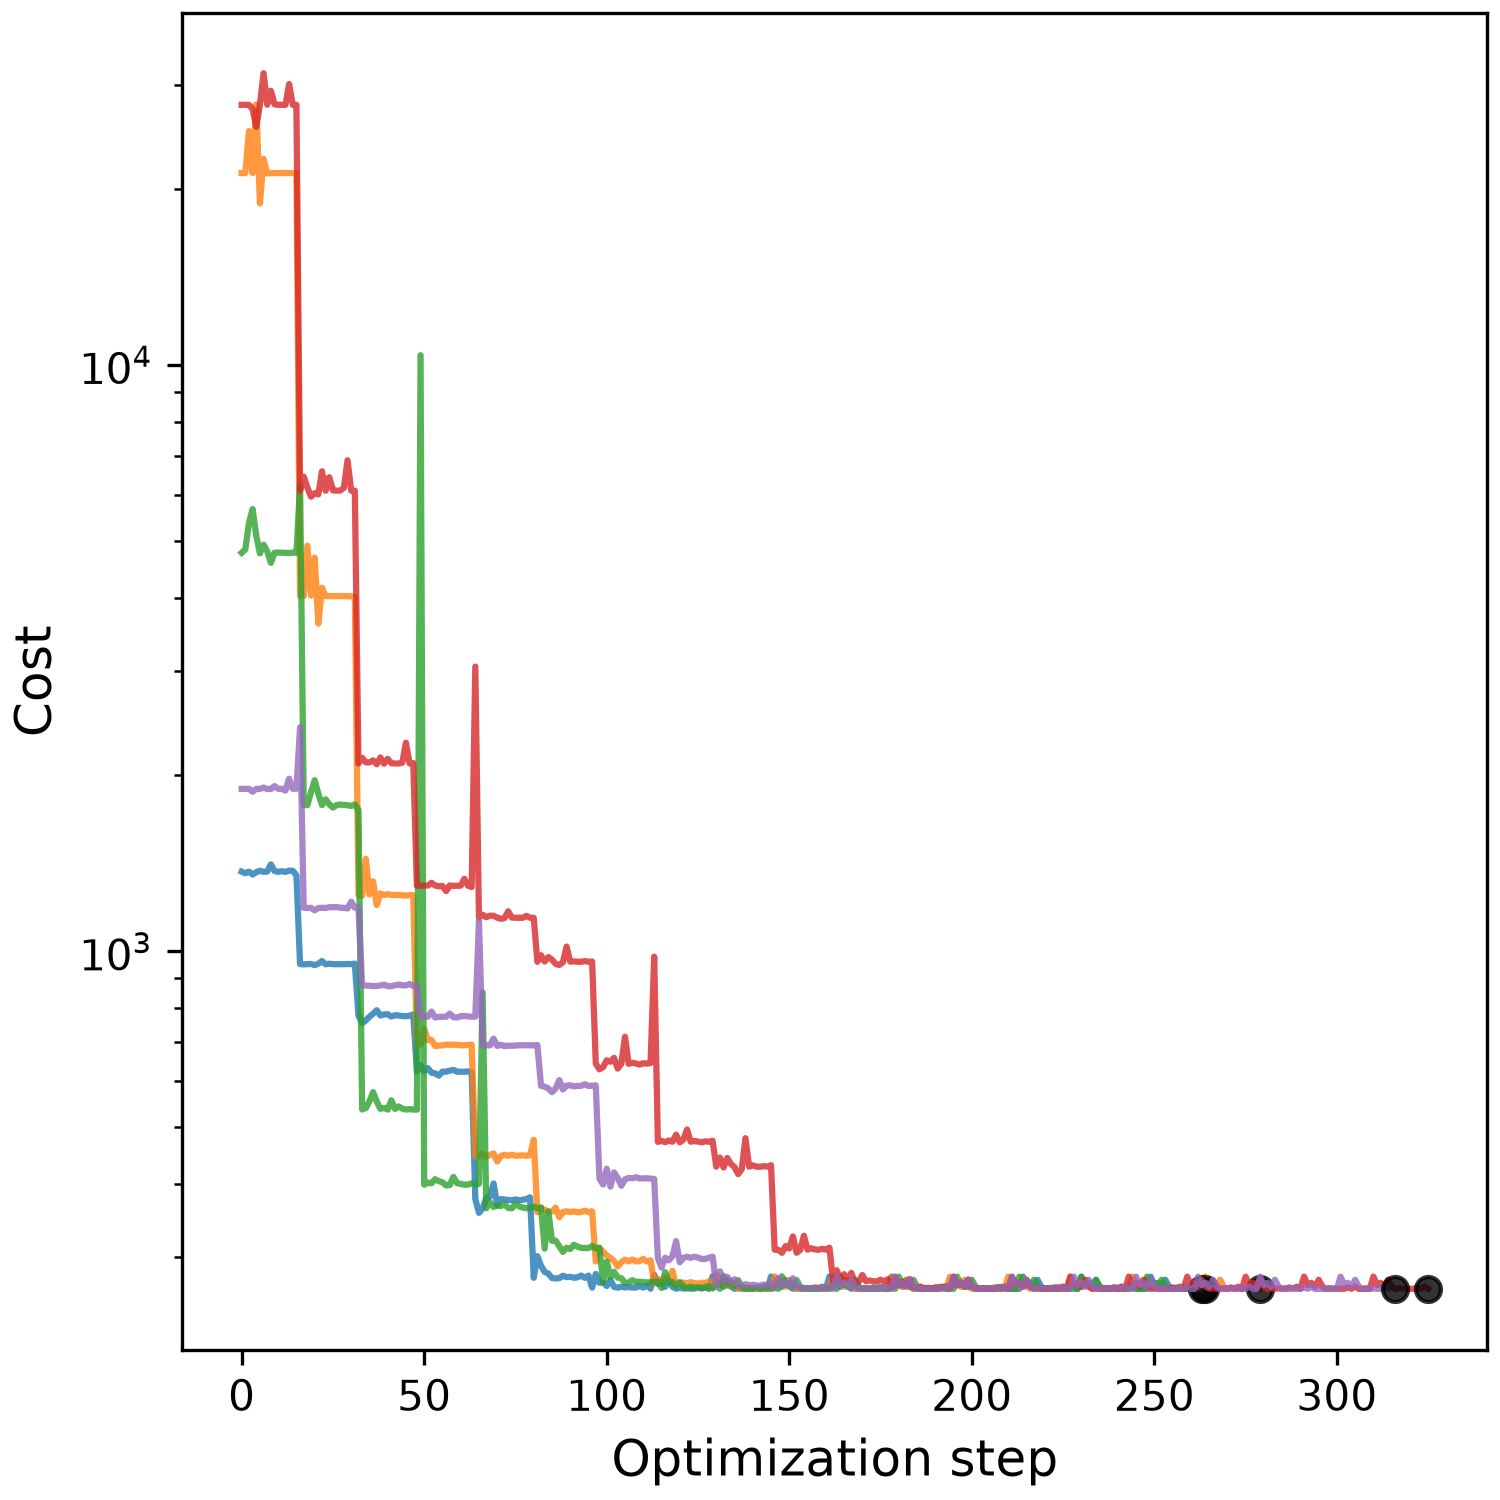
\includegraphics[width=\linewidth]{plots/traces.png}
\caption{Cost of the optimizers over their steps, fit PK\_20261020\_090631\_\_aa2cf. The cost of every optimization run over its steps. Runs which end at the same cost found the same optimum; a run which stops much higher is stuck in a local minimum.}
\label{fig:traces:PK_20261020_090631__aa2cf}
\end{figure}

\begin{figure}[htbp]
\centering
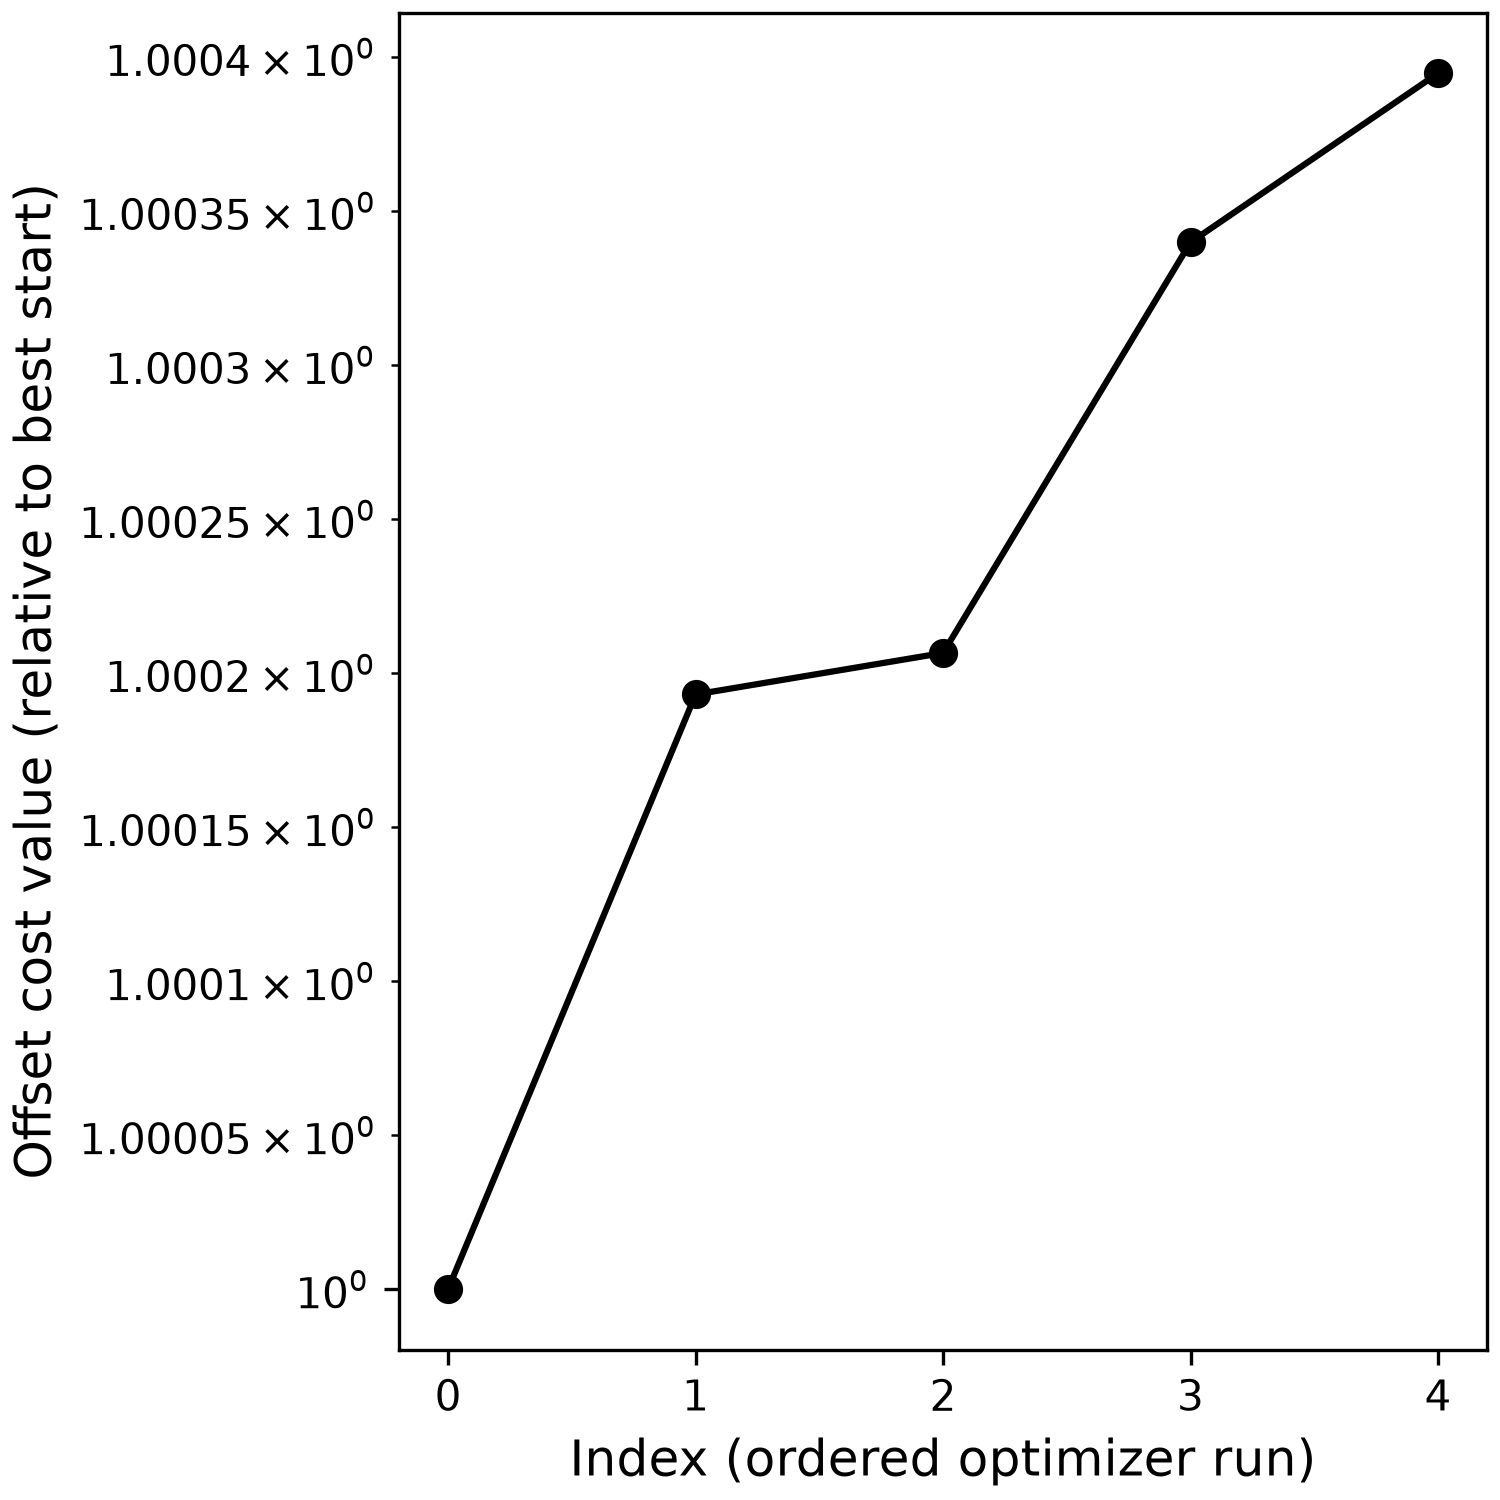
\includegraphics[width=\linewidth]{plots/waterfall.png}
\caption{Cost of the optimization runs, ordered, fit PK\_20261020\_090631\_\_aa2cf. The final cost of the runs, ordered. A flat plateau at the left is the global optimum found repeatedly, which is the evidence that the multistart converged; steps to the right are local minima.}
\label{fig:waterfall:PK_20261020_090631__aa2cf}
\end{figure}

\begin{figure}[htbp]
\centering
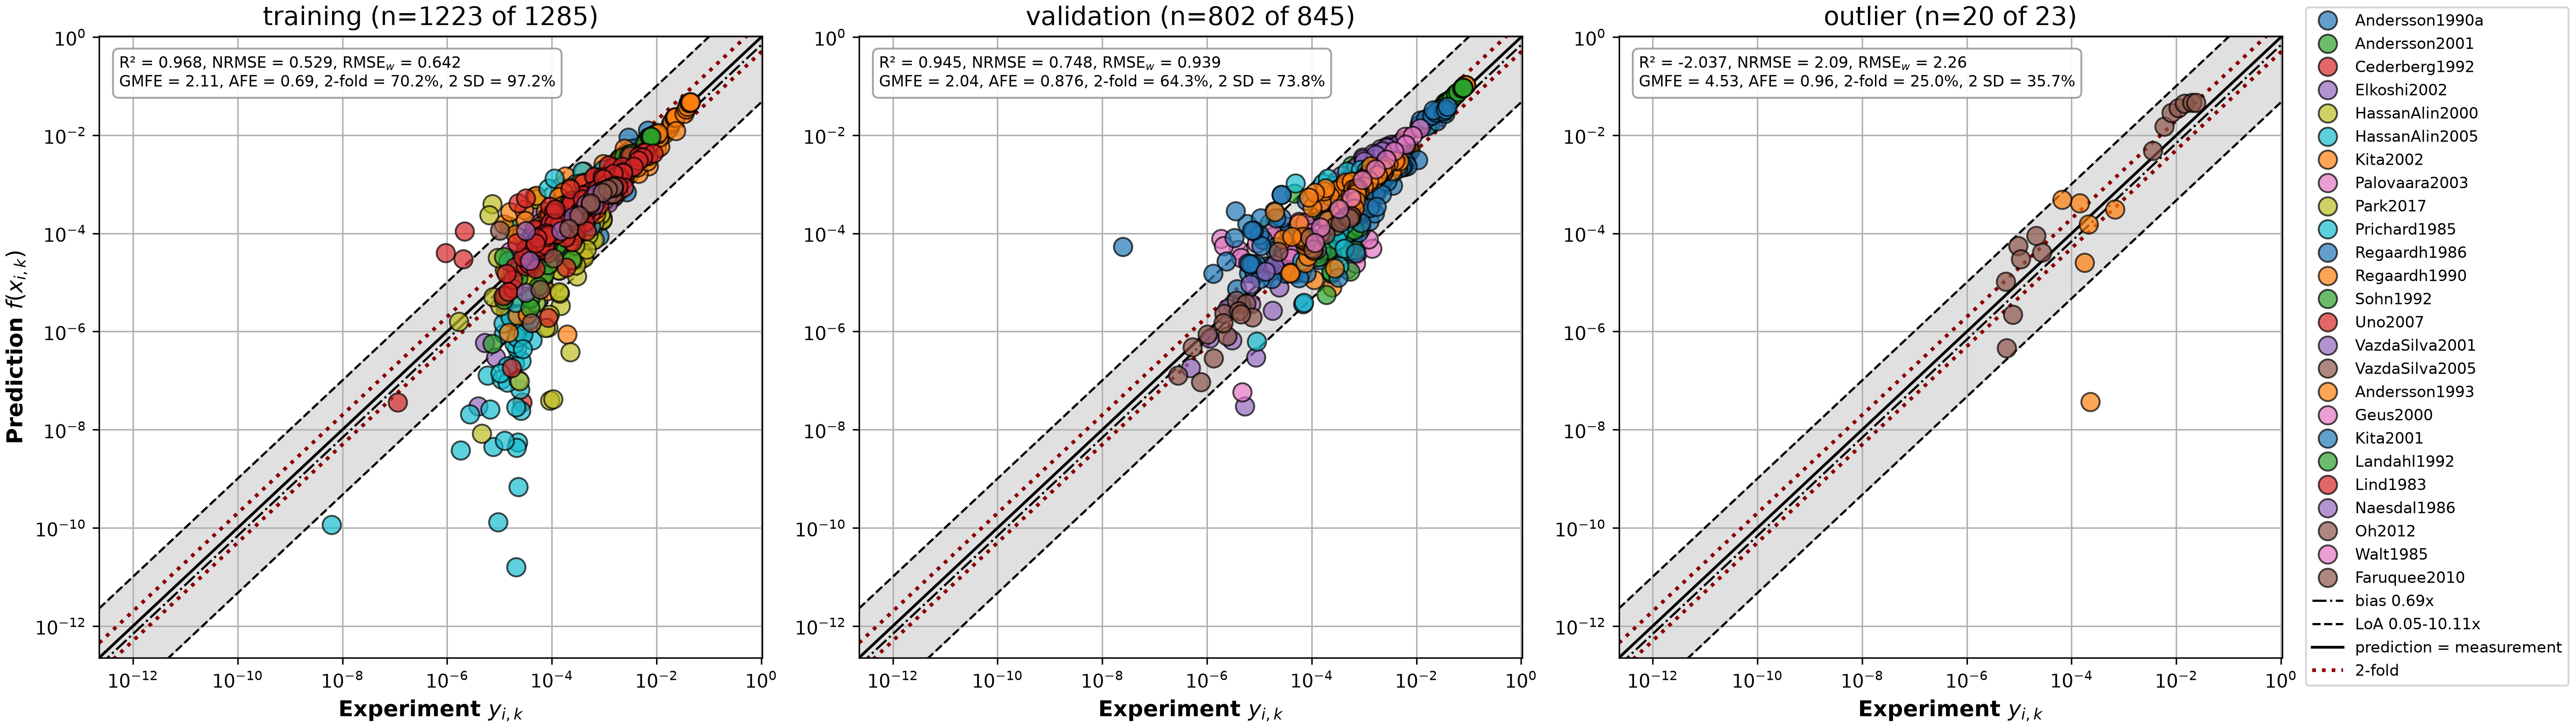
\includegraphics[width=\linewidth]{plots/goodness_of_fit.png}
\caption{Prediction against the measured data points, per kind of fit mapping, with the agreement of the training data, the lines of twofold and the metrics of the panel, fit PK\_20261020\_090631\_\_aa2cf. Within twofold of the data are 859 of the 1223 training data points (70.2\%), 516 of the 802 validation data points (64.3\%) and 5 of the 20 outlier data points (25.0\%); only the data points with a positive value and prediction are counted. Prediction against measurement, one point per data point, with a panel per kind of fit mapping. The points scatter around the diagonal when the model describes the data; a systematic deviation from it is a systematic error of the model. The band is the agreement of the training data, i.e. the same band the Bland-Altman plot draws, here as lines parallel to the diagonal. The dark red dotted lines are twofold, prediction = 2 x measurement and prediction = measurement / 2; the caption states the points between them of every kind. A point which is zero or negative is not drawn on the logarithmic axes and not counted, the title of a panel then states the points drawn of all. The validation panel shows how the fit describes data it was not fitted on, the outlier panel the data the fit dropped. The box of a panel carries its R\ensuremath{^{2}}, its normalized RMSE, the RMSE of the residuals of the cost, its fold errors GMFE and AFE and the percentages of its points within twofold and within two standard deviations of the data.}
\label{fig:goodness_of_fit:PK_20261020_090631__aa2cf}
\end{figure}

\begin{figure}[htbp]
\centering
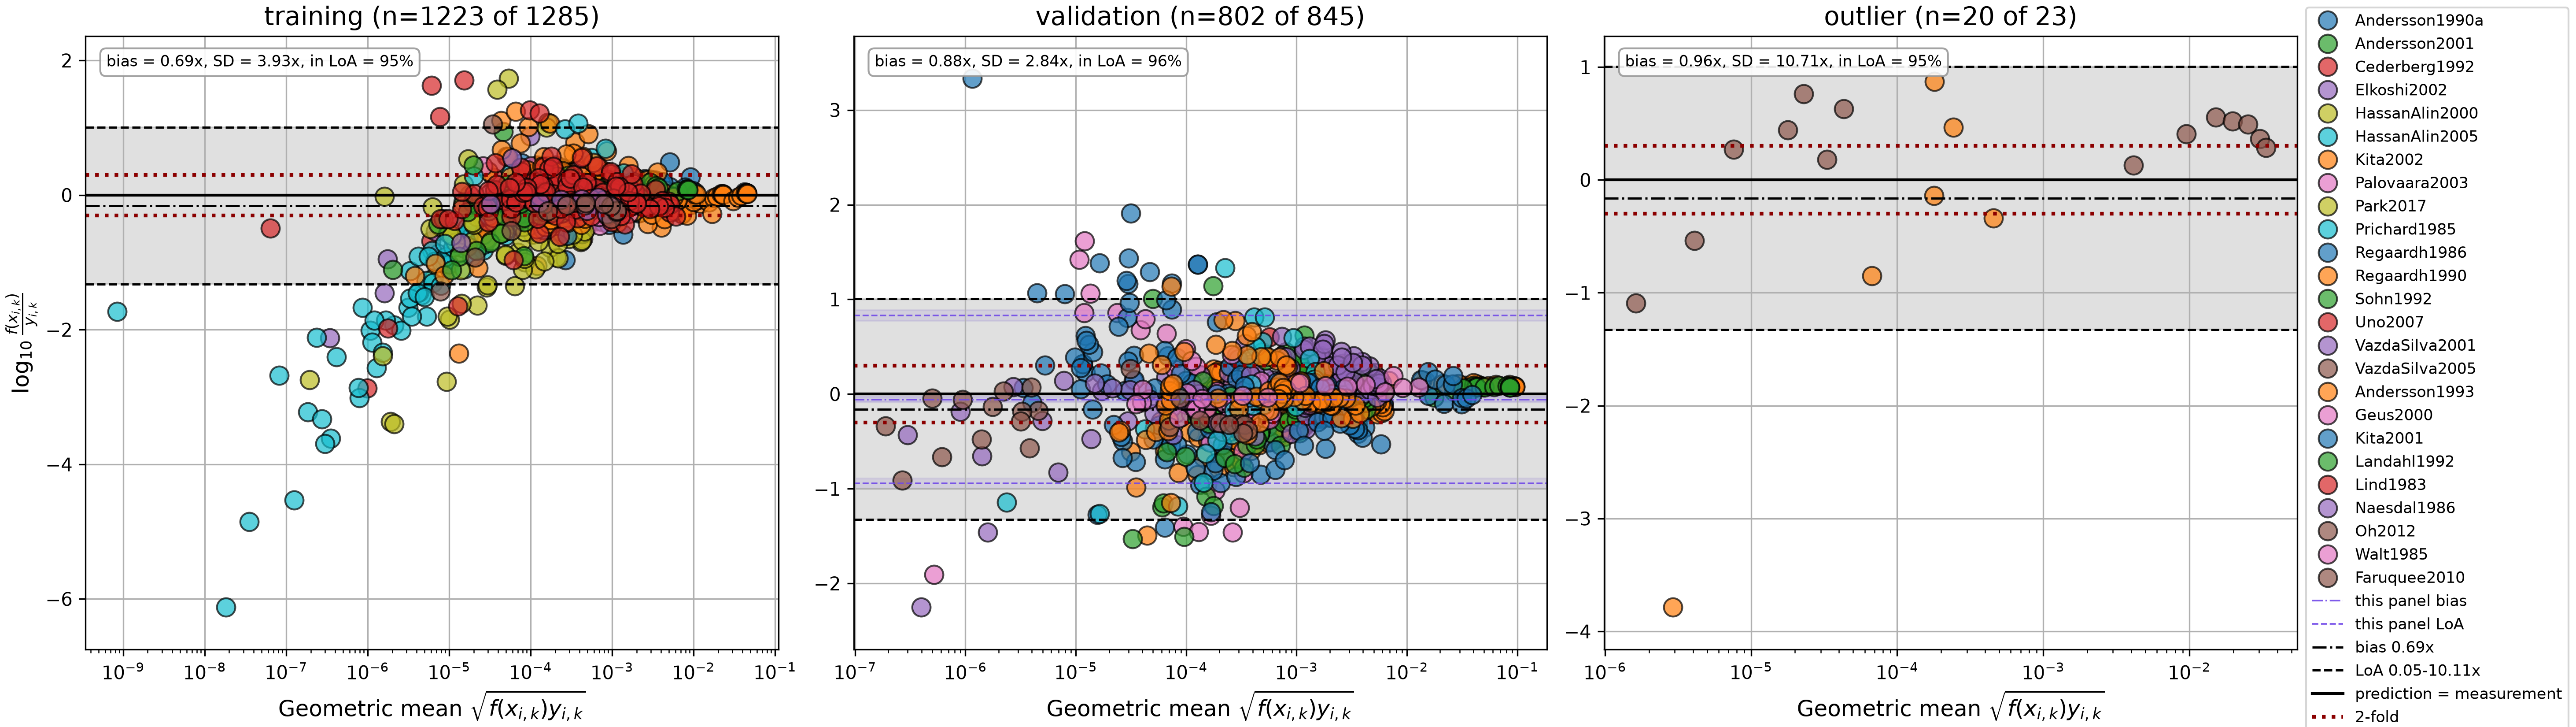
\includegraphics[width=\linewidth]{plots/bland_altman.png}
\caption{Agreement of prediction and measurement as a ratio, per kind of fit mapping, with the agreement of the training data and the agreement of the panel, fit PK\_20261020\_090631\_\_aa2cf. The ratio of prediction and measurement over the geometric mean of the two, i.e. the goodness of fit with the diagonal turned into the horizontal. The band is the same, the bias and the limits of agreement \texttt{bias \ensuremath{\pm} 1.96 SD} of the training data as fold factors. A bias away from 1 is a systematic over- or underprediction, wide limits are a large scatter, and a trend over the mean is a model which describes the large or the small values better. The box of a panel carries the bias and the SD of its own points as fold factors and the share of them inside the limits of agreement of the training data.}
\label{fig:bland_altman:PK_20261020_090631__aa2cf}
\end{figure}

\begin{figure}[htbp]
\centering
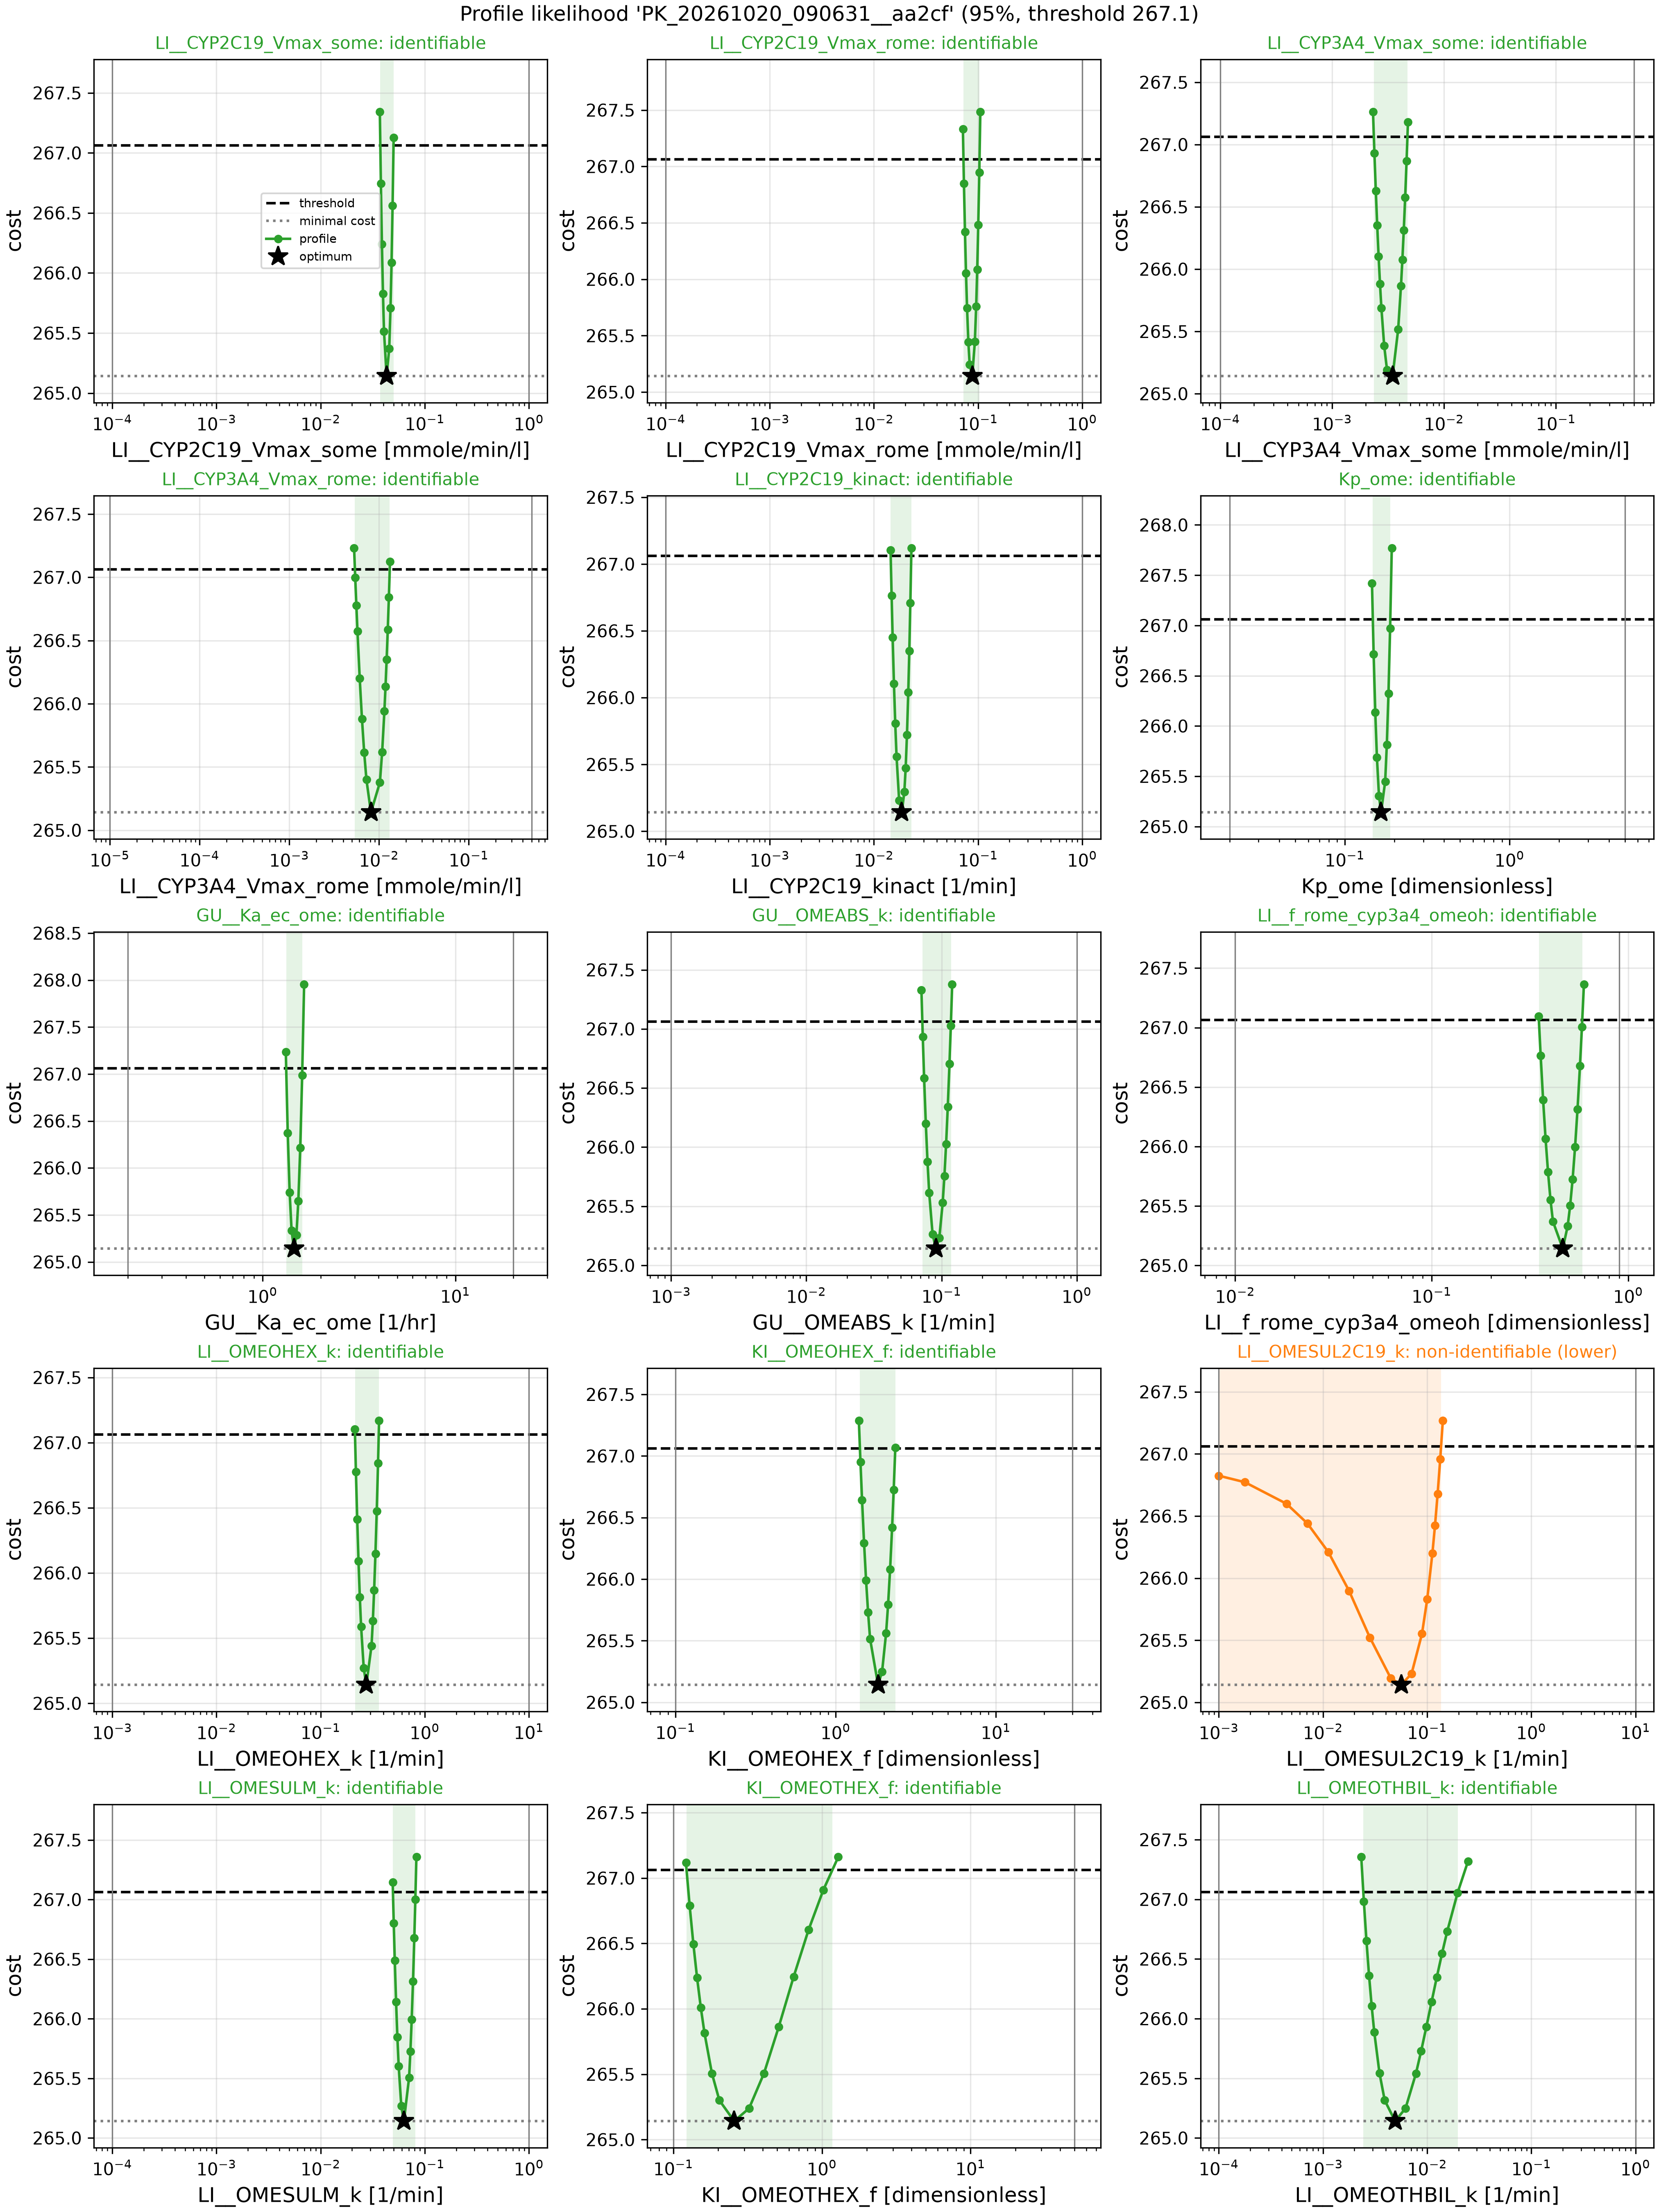
\includegraphics[width=\linewidth]{plots/profiles.png}
\caption{Profile likelihood of every parameter: the cost with the parameter fixed and the other parameters optimized, the threshold of the confidence level and the confidence interval, fit PK\_20261020\_090631\_\_aa2cf. One profile per parameter. A profile which crosses the dashed threshold on both sides gives a finite confidence interval; one which stays below it up to a bound is practically non-identifiable; a flat profile is structurally non-identifiable, the parameter is compensated by the others.}
\label{fig:profiles:PK_20261020_090631__aa2cf}
\end{figure}

\subsection{Provenance}

\begin{longtable}{ll}
\caption{Provenance of the fit PK\_20261020\_090631\_\_aa2cf: the versions it ran with and the revision of its models and data; the SHA-256 checksums of the models and data are listed in Table~\ref{tab:checksums:PK_20261020_090631__aa2cf}.}\label{tab:provenance:PK_20261020_090631__aa2cf} \\
\toprule
Item & Value \\
\midrule
\endfirsthead
\multicolumn{2}{l}{\small\tablename~\thetable{} (continued)} \\
\toprule
Item & Value \\
\midrule
\endhead
\bottomrule
\endlastfoot
Fit & \texttt{PK\_20261020\_090631\_\_aa2cf} \\
Created & 2026-10-20 07:06:37 UTC \\
Seed & 1234 \\
Python & 3.14.4 \\
sbmlsim & 0.10.0 \\
libRoadRunner & 2.10.0 \\
SciPy & 1.18.1 \\
NumPy & 2.5.3 \\
Repository & \texttt{/home/mkoenig/git/pkdb\_models-omeprazole} \\
Commit & \texttt{12acae3ea6826f839295cf826fbb82a2f81d24bd} \\
Uncommitted changes & no \\
\end{longtable}

\bibliographystyle{unsrt}
\bibliography{references}
